\chapter{Вёрстка таблиц} \label{ch:ch3}

\section{Существующие системы управления электроприводом на базе синхронного двигателя с постоянными магнитами
} \label{sec:ch1/sec5}

\subsection{Полеориентированное управление электроприводом на базе синхронного двигателя с постоянными магнитами}
Основные принципы полеориентированного управления были разработаны в 70-х годах девятнадцатого века. Сегодня в результате фундаментальных теоретических исследований и успехов в области силовой полупроводниковой электроники и микропроцессорных систем разработаны электроприводы с векторным управлением, которые серийно выпускаются электротехническими фирмами всего мира. 
Если под скалярным регулированием скорости понимается такое регулирование, при котором в качестве переменных в системе используются эффективные значения напряжений, токов и потокосцеплений, а сами эти величины считаются величинами скалярными, то в основе полеориентированного управления лежит представление об этих величинах, как о пространственных векторах. Можно также отметить, что скалярное управление базируется на зависимостях, лежащих в основе схемы замещения двигателя, а векторное управление — на соответствующих структурных схемах. [35, 27, 117]. 
Для пояснения смысла использования векторного управления обратимся к математическому описанию синхронного двигателя в пространственных векторах при ориентации вещественной оси вращающейся системы координат $d-q$ по вектору ${\Psi }_{2}$ . Такому описанию соответствуют формулы \labelcref{eq:PMSMdqMw} вместе с равенством $\omega_{2эл}=\frac{d \theta_{2}}{d t}$ , выражением для электромагнитного момента и основным уравнением механики. 

\begin{equation}
\label{eq:PMSMdqMw}
\begin{multlined}
\begin{cases}
U_{1 d}=R_{1} i_{1 d}+p\left(L_{1 d} i_{1 d}+\Psi_{2}\right)-\omega_{r} z_{\text{п}}\left(L_{1 q} i_{1 q}\right)
\\
U_{1 q}=R_{1} i_{1 q}+p L_{1 q} i_{1 q}+\omega_{r} z_{\text{п}}\left(L_{1 d} i_{1 d}+\Psi_{2}\right)
\\
M_{\text{э}}=\frac{3}{2} z_{\text{п}}\left(\psi_{1 d} i_{1 q}-\psi_{1 q} i_{1 d}\right)
\\
\frac{d \omega_{r}}{d t}=\frac{1}{J}\left(M_{\text{э}}-M_{\text{с}}\right)
\end{cases}	
\end{multlined}
\end{equation}
где: $\psi_{2 a}=\Psi_{2} \cos \omega t$; $\psi_{2 \beta}=\Psi_{2} \sin \omega t$; $\psi_{1 \alpha}=L_{1} \cdot i_{1 \alpha}+\psi_{2 \alpha}$; $\psi_{1 \beta}=L_{1} \cdot i_{1 \beta}+\psi_{2 \beta}$; $U_{1 \alpha}, U_{1 \beta}, i_{1 \alpha}, i_{1 \beta}, \psi_{1 \alpha}, \psi_{2 \alpha}, \psi_{2 \beta}$ - составляющие векторов напряжений, токов, потокосцеплений по осям $\alpha$ и $\beta$; $r_{1}$, $L_{1}$ - сопротивление, и индуктивность статорной обмотки; $J$ - момент инерции ротора; $\omega_{r}$ – угловая частота вращения ротора; $z_{\text{п}}$ - число пар полюсов двигателя; $M_{\text{э}}$ и $M_{\text{с}}$ - электромагнитный момент и момент статической нагрузки.

\begin{figure}[ht]
	\centering
	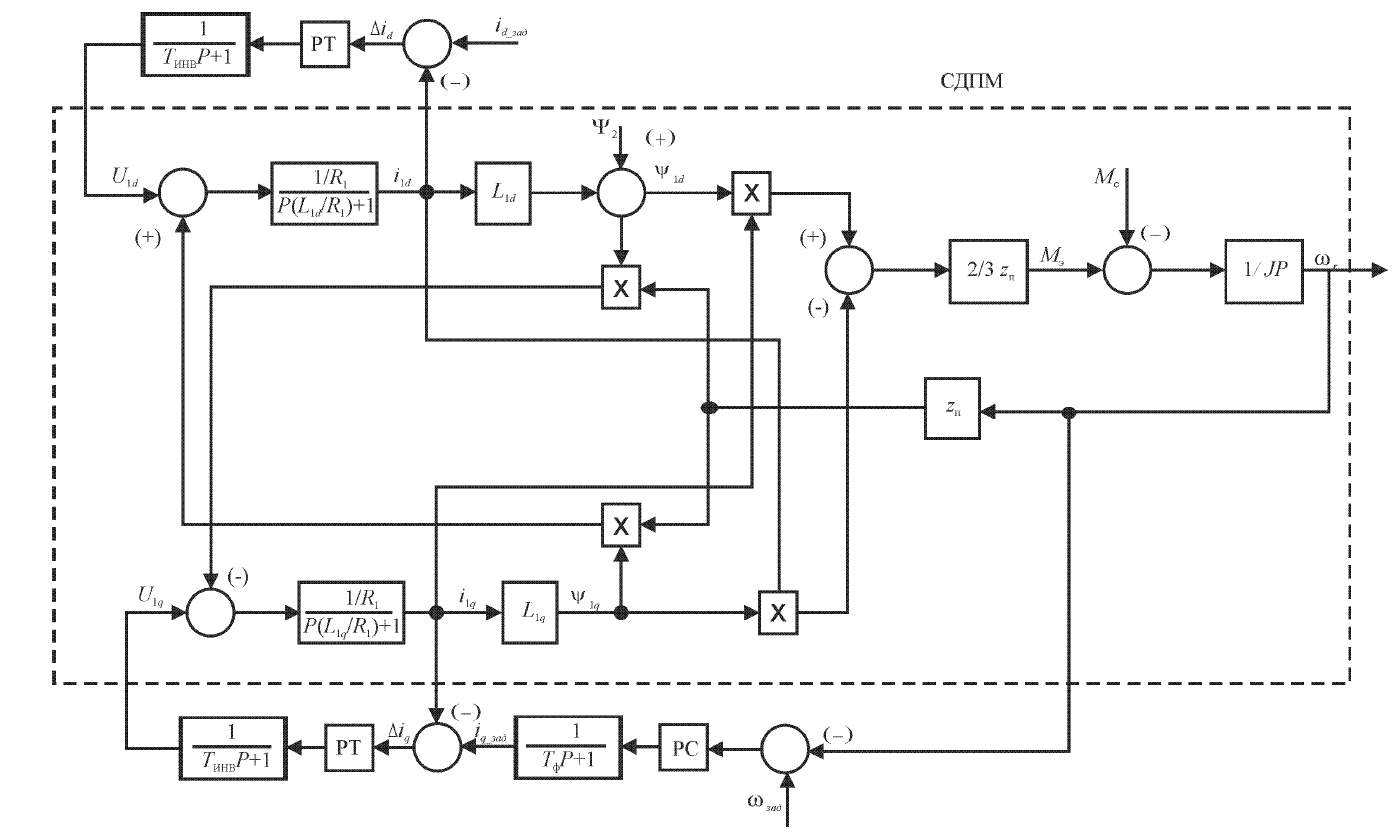
\includegraphics [scale=0.5] {FOCPMSM}
	\caption{Структурная схема электропривода при полеориентированном управлении на базе СДПМ}
	\label{fig:FOCPMSM}
\end{figure}

По этим формулам построена Структурная схема синхронного двигателя (рис. \ref{fig:FOCPMSM}), в которой все переменные представлены сигналами постоянного тока. Входными сигналами являются проекции вектора статорного напряжения $u_{1 d}$ и $u_{1q}$, а выходными величинами электромагнитной части схемы — потокосцепление ротора ${\Psi }_{2}$ и электромагнитный момент $M_{\text{э}}$ . Частота роторной ЭДС $\omega_{r}$ рассчитывается через проекцию на ось $q$ вектора тока статора и потокосцепление ротора. В свою очередь, через скорость двигателя $\omega$ и роторную частоту $\omega_{r}$ рассчитывается частота напряжения обмотки статора $\omega_{\text{эл}}$. В структуре двигателя существуют перекрестные связи между каналом формирования потокосцепления ротора и каналом формирования электромагнитного момента.

Если тем или другим способом скомпенсировать влияние перекрестных связей, то окажется, что сигналом по оси $d$ независимо задается потокосцепление ротора, а сигналом по оси $q$ электромагнитный момент при данном значении потокосцепления ротора ${\Psi }_{2}$. 
Таким образом, структура синхронного двигателя, полученная на основе рассмотрения пространственных векторов, оказывается практически такой же, как структура двигателя постоянного тока независимого возбуждения.
Аналогия с двигателем постоянного тока становится еще более очевидной, если в преобразователе, от которого питается двигатель, с помощью быстродействующих токовых контуров формируются непосредственно составляющие тока статора $i_{1 d}$ и $i_{1 q}$. Улучшение динамических свойств электропривода с синхронным двигателем при векторном управлении является результатом того, что в переходных процессах имеется возможность поддерживать постоянство потокосцепления ротора, в отличие от скалярного регулирования, где потокосцепление ротора в переходных процессах меняется при изменении токов статора и ротора, что приводит к снижению темпа изменения электромагнитного момента. В приводе с полеориентированном управлением, где потокосцепление ротора можно поддерживать постоянным, электромагнитный момент изменяется так быстро, как быстро изменяется составляющая тока статора $i_{1 q}$, (аналогия с изменением момента при изменении тока якоря $i_{\text{я}}$ в машине постоянного тока). 
При первой трактовке [31] к системам с прямой ориентацией по полю относят только те системы, в которых осуществляется непосредственное измерение потока с помощью тех или иных датчиков потока. Вторая трактовка [10, 117] относит к системам с прямой ориентацией и те системы, в которых поток рассчитывается по модели двигателя, так как это даёт возможность, так же как при непосредственном измерении потока, построить замкнутый контур его регулирования. К системам с косвенным измерением в этом случае относят только системы, в которых поток не измеряется и не рассчитывается, а формируется путём задания других переменных. 
Система с косвенной ориентацией по полю не содержит узлов измерения или расчета потокосцепления ротора. Требуемые сигналы задания составляющих тока статора формируются на основании заданных значений потокосцепления ${\Psi }_{2}$ электромагнитного момента. 
Как уже отмечалось, структурная схема синхронного двигателя во вращающейся системе координат содержит в качестве входных и выходных величин проекции соответствующих пространственных векторов на оси вращающейся системы координат. Эти величины являются величинами постоянного тока, что позволяет строить систему управления электроприводом так же, как систему управления электроприводом постоянного тока. Между тем, в реальной системе с трехфазным синхронным двигателем напряжения и токи представляют собой трехфазные системы синусоидальных величин. Поэтому при построении системы управления электроприводом на основе функциональной схемы рис. 2.7. должны быть введены преобразователи координат, осуществляющие преобразование величин постоянного тока во вращающейся системе координат в трехфазную систему величин в неподвижной системе координат и обратно.

\subsection{Прямое управление моментом электроприводом на базе синхронного двигателя с постояными магнитами}

В исследуемой системе прямого управления моментом
СДПМ лежит метод управления моментом и потоком с помощью
предельных циклов путём подачи с выхода инвертора на вход
СДПМ оптимального напряжения.

\noindent Достоинства метода:
\begin{itemize}
	\item хорошие динамические свойства;
	\item простое исполнение.
	\item нет необходимости в использовании прямого преобразователя
	координат, а используется упрощенный обратный преобразователь
	координат;
	\item нет необходимости в использовании датчика скорости;
	\item свойства синхронного электропривода подобны электроприводу постоянного тока с двигателем независимого
	возбуждения
\end{itemize}

\noindent Недостатки метода:
\begin{itemize}
	\item изменяющаяся частота переключения;
	\item точность регулирования определяется используемой моделью двигателя;
	\item большие пульсации токов и момента;
	\item при малых скоростях не обеспечивается стабильный режим
	работы;
	
\end{itemize}

Прямое управление моментом является продолжением и развитием векторного подхода к построению систем управления асинхронным двигателем. Принципы такого управления были опубликованы в 1985 г. и через 10 лет появились первые сообщения о промышленных образцах систем управления фирмы АВВ, построенных на этих принципах.
Задачей прямого управления моментом является обеспечение быстрой реакции электромагнитного момента двигателя на управляющее воздействие. В отличие от полеориентированного управления, где изменение момента производится путем воздействия на ток статора, который, таким образом, является управляемой величиной, в системе с прямым управлением моментом управляемой величиной является потокосцепление статора [1, 2]. Изменение потокосцепления достигается путем оптимального переключения ключей инвертора напряжения, от которого питается синхронный двигатель  (рис. \ref{fig:PMSMDTC}). 

\begin{figure}[ht]
	\centering
	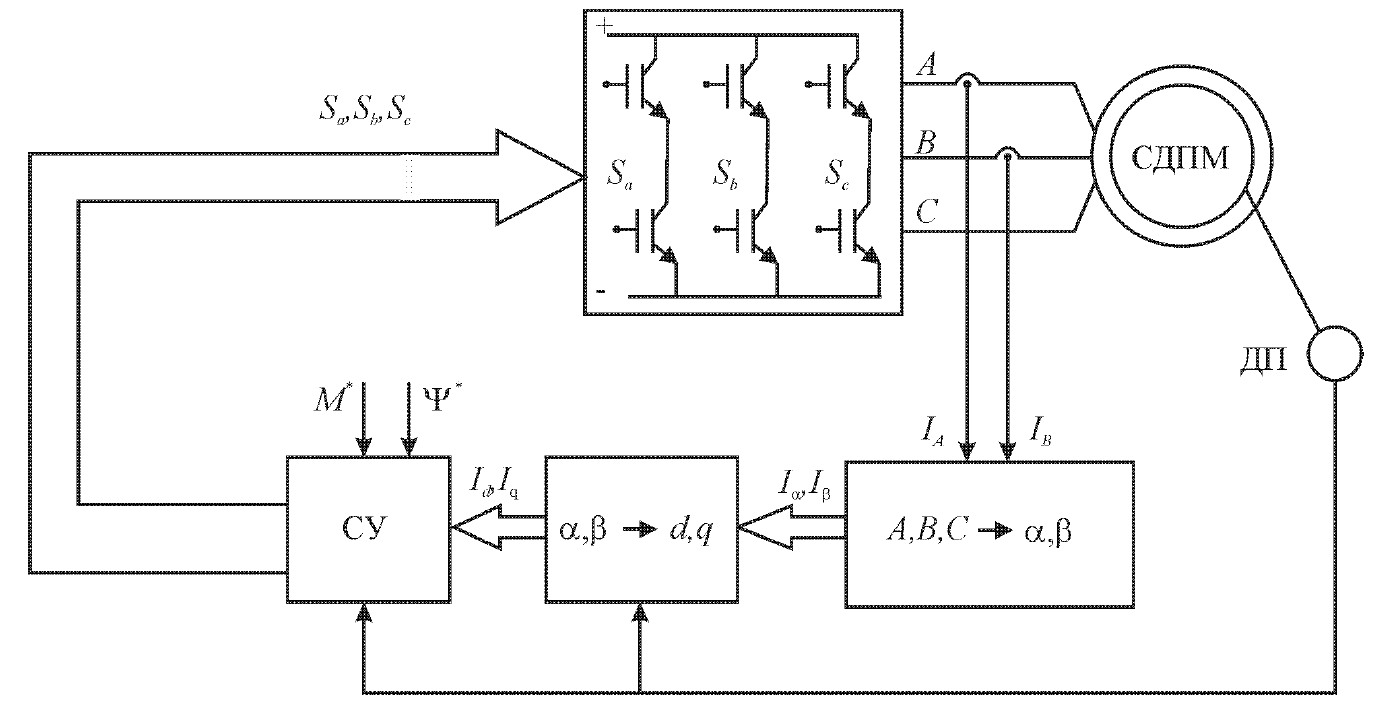
\includegraphics [scale=0.5] {PMSMDTC}
	\caption{Структурная схема электропривода при полеориентированном управлении на базе СДПМ}
	\label{fig:PMSMDTC}
\end{figure}

Для рассмотрения принципа прямого управления моментом [117] могут быть использованы два полученных ранее выражения: уравнение равновесия напряжений статорной цепи в неподвижной системе координат (формула \ref{eq:U1dq}) и выражение \ref{eq:Mel} для электромагнитного момента двигателя. 
\begin{equation}
\label{eq:U1dq}
\overline{U}_{\mathrm{ldq}}=R_{1} \overline{I}_{\mathrm{ldq}}+\frac{d}{d t} \overline{\Psi}_{\mathrm{ldq}}
\end{equation}
\begin{equation}
\label{eq:Mel}
\vec{M}_{\text{э}}=L_{1}\left(\vec{\Psi}_{1} \Psi_{2}^{*}\right)
\end{equation}
Это выражение, в котором момент рассчитывается через потокосцепления статора и ротора, записано во вращающейся системе координат d-q, но поскольку значение момента не зависит от выбора системы координат, в которой рассматриваются векторы $\overline{\Psi}_{1}$ и $\overline{\Psi}_{2}$ , то оно может быть представлено в неподвижной системе координат $d-q$ в виде:
\begin{equation}
M_{\text{э}}=\frac{3}{2} z_{\text{п}} L_{1}\left(\psi_{1 q} \psi_{2 d}-\psi_{1 d} \psi_{2 q}\right)
\end{equation}

На рис. \ref{fig:VectorPMSM} [3, 117] показана координатная плоскость, на которой отмечены оси неподвижной системы координат $d-q$ и расположение векторов напряжения и потокосцепления статора. Плоскость поделена на шесть секторов I — VI по 60 эл. град каждый.

\begin{figure}[ht]
	\centering
	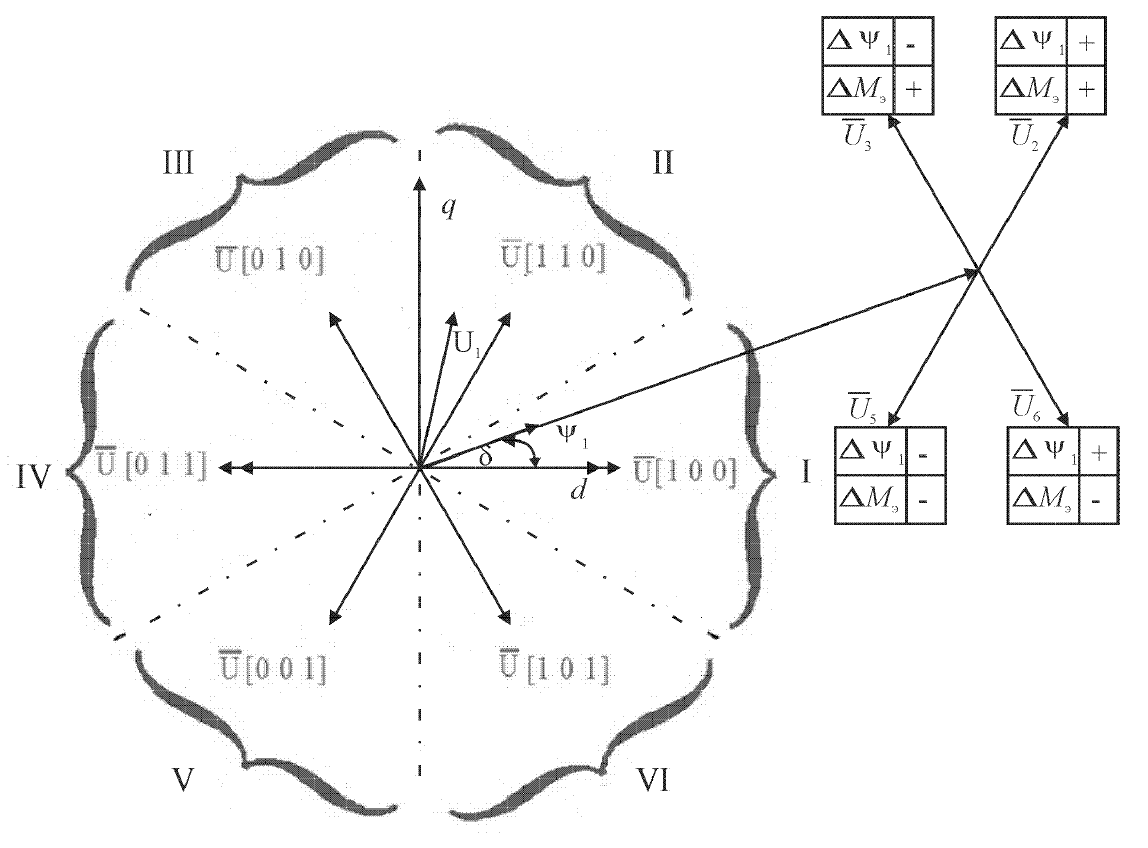
\includegraphics [scale=0.5] {VectorPMSM}
	\caption{Структурная схема электропривода при полеориентированном управлении на базе СДПМ}
	\label{fig:VectorPMSM}
\end{figure}

Пространственный вектор напряжения на выходе инвертора, от которого питается обмотка статора двигателя, может занимать одно из шести фиксированных ненулевых положений и два
нулевых положения. Ненулевые векторы $\overline{U}_{1}-\overline{U}_{6}$ и нулевые, обозначаемые, как $\overline{U}_{7}-\overline{U}_{7}$ , рассматриваются как самостоятельные базовые векторы. На рис. \ref{fig:VectorPMSM} показано мгновенное положение вектора потокосцепления статора, который в данный момент времени находится в секторе I.

Таким образом, для организации прямого управления моментом необходимо знать текущие значения потокосцепления статора и момента двигателя.

Для расчета значений потокосцепления статора и электромагнитного момента необходимо располагать проекциями векторов тока и напряжения в системе координат $d-q$. Поэтому в модели выполняется преобразование симметричной трехфазной системы токов и напряжений в проекции соответствующих векторов на оси неподвижной системы координат (см. рис. \ref{fig:VectorPMSM}). 
Сравнительный анализ электроприводов на базе синхронного двигателя с постоянными магнитами с системой полеориентированного управления и системой прямого управления
моментом показал, что обе системы управления применимы в электроприводах при различных требованиях к показателям регулируемого электропривода в различных режимах работы со стороны технологического процесса [1].

\section{Сошлёмся на библиографию} \label{sec:ch1/sec4}


Сошлёмся на библиографию.
Одна ссылка: \cite[с.~54]{Sokolov}\cite[с.~36]{Gaidaenko}.
Две ссылки: \cite{Sokolov,Gaidaenko}.
Много ссылок: %\cite[с.~54]{Lermontov,Management,Borozda} % такой «фокус»
%вызывает biblatex warning относительно опции sortcites, потому что неясно, к
%какому источнику относится уточнение о страницах, а bibtex об этой проблеме
%даже не предупреждает
\cite{Lermontov, Management, Borozda, Marketing, Constitution, FamilyCode,
	Gost.7.0.53, Razumovski, Lagkueva, Pokrovski, Methodology, Nasirova, Berestova,
	Kriger}%
\ifnumequal{\value{bibliosel}}{0}{% Примеры для bibtex8
	\cite{Sirotko, Lukina, Encyclopedia}%
}{% Примеры для biblatex через движок biber
	\cite{Sirotko2, Lukina2, Encyclopedia2}%
}%
.
И~ещё немного ссылок:
\cite{Article,Book,Booklet,Conference,Inbook,Incollection,Manual,Mastersthesis,
	Misc,Phdthesis,Proceedings,Techreport,Unpublished}
% Следует обратить внимание, что пробел после запятой внутри \cite{}
% обрабатывается ожидаемо, а пробел перед запятой, может вызывать проблемы при
% обработке ссылок.
\cite{medvedev2006jelektronnye, CEAT:CEAT581, doi:10.1080/01932691.2010.513279,
	Gosele1999161,Li2007StressAnalysis, Shoji199895, test:eisner-sample,
	test:eisner-sample-shorted, AB_patent_Pomerantz_1968, iofis_patent1960}
\ifnumequal{\value{bibliosel}}{0}{% Примеры для bibtex8
}{% Примеры для biblatex через движок biber
	\cite{patent2h, patent3h, patent2}%
}%
.

\ifnumequal{\value{bibliosel}}{0}{% Примеры для bibtex8
	Попытка реализовать несколько ссылок на конкретные страницы
	для \texttt{bibtex} реализации библиографии:
	[\citenum{Sokolov}, с.~54; \citenum{Gaidaenko}, с.~36].
}{% Примеры для biblatex через движок biber
	Несколько источников (мультицитата):
	% Тут специально написано по-разному тире, для демонстрации, что
	% применение специальных тире в настоящий момент в biblatex приводит к непоказу
	% "с.".
	\cites[vii--x, 5, 7]{Sokolov}[v"--~x, 25, 526]{Gaidaenko}[vii--x, 5, 7]{Techreport},
	работает только в \texttt{biblatex} реализации библиографии.
}%

Ссылки на собственные работы:~\cite{vakbib1, confbib1}

Сошлёмся на приложения: Приложение \ref{app:A}, Приложение \ref{app:B2}.

Сошлёмся на формулу: формула \eqref{eq:equation1}.

Сошлёмся на изображение: рисунок \ref{fig:knuth}.

Стандартной практикой является добавление к ссылкам префикса, характеризующего тип элемента.
Это не является строгим требованием, но позволяет лучше ориентироваться в документах большого размера.
Например, для ссылок на рисунки используется префикс \textit{fig},
для ссылки на таблицу -- \textit{tab}.

В таблице \ref{tab:tab_pref} приложения \ref{app:B4} приведён список рекомендуемых
к использованию стандартных префиксов.

\section{Формулы} \label{sec:ch1/sec0}











\section{Одиночное изображение} \label{sec:ch2/sec1}

\begin{figure}[ht]
	\centering
	\includegraphics [scale=0.27] {latex}
	\caption{TeX.}
	\label{fig:latex}
\end{figure}



\section{Длинное название параграфа, в котором мы узнаём как сделать две картинки с~общим номером и названием} \label{sec:ch2/sect2}

А это две картинки под общим номером и названием:
\begin{figure}[ht]
	\begin{minipage}[ht]{0.49\linewidth}\centering
		\includegraphics[width=0.5\linewidth]{knuth1} \\ а)
	\end{minipage}
	\hfill
	\begin{minipage}[ht]{0.49\linewidth}\centering
		\includegraphics[width=0.5\linewidth]{knuth2} \\ б)
	\end{minipage}
	\caption{Очень длинная подпись к изображению,
		на котором представлены две фотографии Дональда Кнута}
	\label{fig:knuth}
\end{figure}

Те~же~две картинки под~общим номером и~названием,
но с автоматизированной нумерацией подрисунков:
\begin{figure}[ht]
	{\centering
		\hfill
		\subbottom[List-of-Figures entry][Первый подрисунок\label{fig:knuth_2-1}]{%
			\includegraphics[width=0.25\linewidth]{knuth1}}
		\hfill
		\subbottom[\label{fig:knuth_2-2}]{%
			\includegraphics[width=0.25\linewidth]{knuth2}}
		\hfill
		\subbottom[Третий подрисунок]{%
			\includegraphics[width=0.3\linewidth]{example-image-c}}
		\hfill
	}
	\legend{Подрисуночный текст, описывающий обозначения, например. Согласно
		ГОСТ 2.105, пункт 4.3.1, располагается перед наименованием рисунка.}
	\caption[Этот текст попадает в названия рисунков в списке рисунков]{Очень
		длинная подпись к второму изображению, на~котором представлены две
		фотографии Дональда Кнута}
	\label{fig:knuth_2}
\end{figure}

На рисунке~\ref{fig:knuth_2-1} показан Дональд Кнут без головного убора.
На рисунке~\ref{fig:knuth_2}\subcaptionref*{fig:knuth_2-2}
показан Дональд Кнут в головном уборе.

Возможно вставлять векторные картинки, рассчитываемые \LaTeX\ <<на~лету>>
с~их~предварительной компиляцией. Надписи в таких рисунках будут выполнены
тем же~шрифтом, который указан для документа в целом.
На~рисунке~\ref{fig:tikz_example} на~странице~\pageref{fig:tikz_example}
представлен пример схемы, рассчитываемой пакетом \verb|tikz| <<на~лету>>.
Для ускорения компиляции, подобные рисунки могут быть <<кешированы>>, что
определяется настройками в~\verb|common/setup.tex|.
Причём имя предкомпилированного
файла и~папка расположения таких файлов могут быть отдельно заданы,
что удобно, если не~для подготовки диссертации,
то~для подготовки научных публикаций.
\begin{figure}[ht]
	{\centering
		\ifdefmacro{\tikzsetnextfilename}{\tikzsetnextfilename{tikz_example_compiled}}{}% присваиваемое предкомпилированному pdf имя файла
		\input{Dissertation/images/tikz_scheme.tikz}
		
	}
	\legend{}
	\caption[Пример \texttt{tikz} схемы]{Пример рисунка, рассчитываемого
		\texttt{tikz}, который может быть предкомпилирован}
	\label{fig:tikz_example}
\end{figure}

Множество программ имеют либо встроенную возможность экспортировать векторную
графику кодом \verb|tikz|, либо соответствующий пакет расширения.
Например, в GeoGebra есть встроенный экспорт,
для Inkscape есть пакет svg2tikz,
для Python есть пакет matplotlib2tikz,
для R есть пакет tikzdevice.

\section{Пример вёрстки списков} \label{sec:ch2/sec3}

\noindent Нумерованный список:
\begin{enumerate}
	\item Первый пункт.
	\item Второй пункт.
	\item Третий пункт.
\end{enumerate}

\noindent Маркированный список:
\begin{itemize}
	\item Первый пункт.
	\item Второй пункт.
	\item Третий пункт.
\end{itemize}

\noindent Вложенные списки:
\begin{itemize}
	\item Имеется маркированный список.
	\begin{enumerate}
		\item В нём лежит нумерованный список,
		\item в котором
		\begin{itemize}
			\item лежит ещё один маркированный список.
		\end{itemize}
	\end{enumerate}
\end{itemize}

\noindent Нумерованные вложенные списки:
\begin{enumerate}
	\item Первый пункт.
	\item Второй пункт.
	\item Вообще, по ГОСТ 2.105 первый уровень нумерации
	(при необходимости ссылки в тексте документа на одно из перечислений)
	идёт буквами русского или латинского алфавитов,
	а второй "--- цифрами со~скобками.
	Здесь отходим от ГОСТ.
	\begin{enumerate}
		\item в нём лежит нумерованный список,
		\item в котором
		\begin{enumerate}
			\item ещё один нумерованный список,
			\item третий уровень нумерации не нормирован ГОСТ 2.105;
			\item обращаем внимание на строчность букв,
			\item в этом списке
			\begin{itemize}
				\item лежит ещё один маркированный список.
			\end{itemize}
		\end{enumerate}
		
	\end{enumerate}
	
	\item Четвёртый пункт.
\end{enumerate}

\section{Традиции русского набора}

Много полезных советов приведено в материале
<<\href{http://www.dropbox.com/s/x4hajy4pkw3wdql/wholesome-typesetting.pdf?dl=1\&pv=1}{Краткий курс благородного набора}>> (автор А.\:В.~Костырка).
Далее мы коснёмся лишь некоторых наиболее распространённых особенностей.

\subsection{Пробелы}

В~русском наборе принято:
\begin{itemize}
	\item единицы измерения, знак процента отделять пробелами от~числа:
	10~кВт, 15~\% (согласно ГОСТ 8.417, раздел 8);
	\item $\tg 20\text{\textdegree}$, но: 20~{\textdegree}C
	(согласно ГОСТ 8.417, раздел 8);
	\item знак номера, параграфа отделять от~числа: №~5, \S~8;
	\item стандартные сокращения: т.\:е., и~т.\:д., и~т.\:п.;
	\item неразрывные пробелы в~предложениях.
\end{itemize}

\subsection{Математические знаки и символы}

Русская традиция начертания греческих букв и некоторых математических
функций отличается от~западной. Это исправляется серией
\verb|\renewcommand|.
\begin{itemize}
	%Все \original... команды заранее, ради этого примера, определены в Dissertation\userstyles.tex
	\item[До:] \( \originalepsilon \originalge \originalphi\),
	\(\originalphi \originalleq \originalepsilon\),
	\(\originalkappa \in \originalemptyset\),
	\(\originaltan\),
	\(\originalcot\),
	\(\originalcsc\).
	\item[После:] \( \epsilon \ge \phi\),
	\(\phi \leq \epsilon\),
	\(\kappa \in \emptyset\),
	\(\tan\),
	\(\cot\),
	\(\csc\).
\end{itemize}

Кроме того, принято набирать греческие буквы вертикальными, что
решается подключением пакета \verb|upgreek| (см. закомментированный
блок в~\verb|userpackages.tex|) и~аналогичным переопределением в
преамбуле (см.~закомментированный блок в~\verb|userstyles.tex|). В
этом шаблоне такие переопределения уже включены.

Знаки математических операций принято переносить. Пример переноса
в~формуле \eqref{eq:equation3}.

\subsection{Кавычки}
В английском языке приняты одинарные и двойные кавычки в~виде ‘...’ и~“...”.
В России приняты французские («...») и~немецкие („...“) кавычки (они называются
«ёлочки» и~«лапки», соответственно). ,,Лапки`` обычно используются внутри
<<ёлочек>>, например, <<... наш гордый ,,Варяг``...>>.

Французкие левые и правые кавычки набираются
как лигатуры \verb|<<| и~\verb|>>|, а~немецкие левые
и правые кавычки набираются как лигатуры \verb|,,| и~\verb|‘‘| (\verb|``|).

Вместо лигатур или команд с~активным символом "\ можно использовать команды
\verb|\glqq| и \verb|\grqq| для набора немецких кавычек и команды \verb|\flqq|
и~\verb|\frqq| для набора французских кавычек. Они определены в пакете
\verb|babel|.

\subsection{Тире}
%  babel+pdflatex по умолчанию, в polyglossia надо включать опцией (и перекомпилировать с удалением временных файлов)
Команда \verb|"---| используется для печати тире в тексте. Оно несколько короче
английского длинного тире. Кроме того, команда задаёт небольшую жёсткую отбивку
от слова, стоящего перед тире. При этом, само тире не~отрывается от~слова.
После тире следует такая же отбивка от текста, как и~перед тире. При наборе
текста между словом и командой, за которым она следует, должен стоять пробел.

В составных словах, таких, как <<Закон Менделеева"--~Клапейрона>>, для печати
тире надо использовать команду \verb|"--~|. Она ставит более короткое,
по~сравнению с~английским, тире и позволяет делать переносы во втором слове.
При~наборе текста команда \verb|"--~| не отделяется пробелом от слова,
за~которым она следует (\verb|Менделеева"--~|). Следующее за командой слово
может быть  отделено от~неё пробелом или перенесено на другую строку.

Если прямая речь начинается с~абзаца, то перед началом её печатается тире
командой \verb|"--*|. Она печатает русское тире и жёсткую отбивку нужной
величины перед текстом.

\subsection{Дефисы и переносы слов}
%  babel+pdflatex по умолчанию, в polyglossia надо включать опцией (и перекомпилировать с удалением временных файлов)
Для печати дефиса в~составных словах введены две команды. Команда~\verb|"~|
печатает дефис и~запрещает делать переносы в~самих словах, а~команда \verb|"=|
печатает дефис, оставляя \TeX ’у право делать переносы в~самих словах.

В отличие от команды \verb|\-|, команда \verb|"-| задаёт место в~слове, где
можно делать перенос, не~запрещая переносы и~в~других местах слова.

Команда \verb|""| задаёт место в~слове, где можно делать перенос, причём дефис
при~переносе в~этом месте не~ставится.

Команда \verb|",| вставляет небольшой пробел после инициалов с~правом переноса
в~фамилии.

\section{Текст из панграмм и формул}